\chapter{Introdução} \label{cap:introducao}

Neste capítulo iremos apresentar o contexto da pesquisa, sua motivação, o
objetivo da mesma e como este trabalho está organizado.

\section{Contexto e Motivação}
 
A natureza da engenharia de requisitos envolve uma margem ampla de
\textit{stakeholders}: usuários, clientes, desenvolvedores, gerentes de projeto,
mantenedores e assim por diante.  Eles são responsáveis por decidir conjuntamente, o que fazer, quando fazê-lo, quais informações são necessárias e finalmente,
como fazer. Essa ideia é apresentada por Sommerville I. e Sawyer P
em \cite{Sommerville:1997:REG:549198}.

Não é difícil imaginar, portanto, um
executivo que necessita de um \textit{software} para sua empresa, visando diminuir custos. Um exemplo simples, mas que serve à nosso propósito de contextualização, é um sistema de gerenciamento
de estoque. Esse mesmo indivíduo pensa em conseguir tal objeto de desejo de
maneira mais fácil, com menor custo, no menor tempo e com melhor qualidade.

Pensemos agora, em um gerente de projeto, que
precisa analisar diariamente cronogramas, gastos e seus subordinados. Para este
indivíduo, a clareza das tarefas e a facilidade de atribuí-las a alguém são
verdadeiros pontos relevantes, como também a capacidade de sua equipe.
Um usuário, talvez um vendedor da empresa do executivo
mencionado acima, precisa unicamente que o sistema seja intuitivo, que responda
aos seus comandos e que não seja difícil de usar, afinal ele precisa realizar
seu trabalho e não quer que uma ferramenta o atrapalhe.
Um ou mais desenvolvedores irão programar, a fim de que o \textit{software} seja criado.
Podemos entender que um dos objetivos destes é ter menos tarefas para realizar,
por meio de reuso de código.
Por fim, existe ainda o executivo da empresa contratada para entregar o
\textit{software}, no qual o gerente de projeto e os desenvolvedores trabalham,
quer que o projeto acabe o mais rápido, porém que ele obtenha maior lucro.

Segundo Arthur Schopenhauer em \cite{as1860}, o homem é movido pela ideia de
``tudo para mim e nada para os outros'', esse é portanto o princípio básico do
egoísmo, pensar que podemos desfrutar de tudo e possuir tudo; mas, como isso é
impossível, querer, pelo menos, dominar tudo. Desta forma, com os diferentes
objetivos apresentados para os \textit{stakeholders}, é fácil entender que
conflitos são eventos comuns no dia a dia \cite{Barki:2001:ICM:2017138.2017142}.

Gustave Le Bon em \cite{lebon1954} diz, por outro lado, que ``quaisquer que
sejam os indivíduos que compõem uma massa (grupo de indivíduos), sejam semelhantes ou dessemelhantes o seu tipo de vida, suas
ocupações, seu caráter ou sua inteligência, o simples fato de se terem
transformado em massa os torna possuidores de uma espécie de alma coletiva. Esta
alma os faz sentir, pensar e agir de uma forma bem diferente da que cada um sentiria, pensaria e agiria isoladamente.''.

Podemos entender que quando os \textit{stakeholders} se juntam para debater
sobre o processo de \textit{software}, eles querem coisas bem diferentes, mas
quando laços são estabelecidos, eventualmente eles se empenharão em negociar. A maneira que a
negociação é feita depende da intensidade desses laços, quais
\textit{stakeholders} o possuem e de quando e por que eles seriam rompidos.

 A negociação é, então, primordial para o sucesso do projeto e existem diversas
 formas de conduzi-la, conhecidas como técnicas de negociação de requisitos.
 Para entender melhor este conceito, no contexto deste trabalho, criamos uma
 definição para o que é uma técnica e uma definição para o que é negociação,
 além disso usaremos a definição de requisito apresentada por Pfleeger
 em \cite{Pfleeger:2004:SET:517000}. Dessa forma podemos construir a definição
 de o que é uma técnica de negociação de requisitos.

-Técnica é um conjunto de
passos, métodos e regras aplicadas a um processo executável.

-Negociação é um processo executável pela qual duas ou mais pessoas buscam o
entendimento, consenso e a construção de acordos para eliminar ou minimizar suas diferenças.

-Um requisito é uma característica do sistema ou a descrição de algo que o.
sistema é capaz de realizar para atingir os seus objetivos

Portanto, tomemos como definição, que técnica de Negociação
de Requisitos é um conjunto de passos, métodos e regras, que são aplicadas por
duas ou mais pessoas, buscando o entendimento, consenso e a construção de
acordos para eliminar ou minimizar suas diferenças, referentes as suas interpretações sobre as características de um sistema ou a descrição de algo que o sistema é capaz de realizar para atingir os seus objetivos.

Essas interpretações, em um contexto de desenvolvimento de \textit{software},
podem se referir ao custo dos requisitos, ao prazo para que eles sejam atendidos, ao
escopo ou aos atributos de qualidade. Nesta situação, podem haver conflitos que
por si só possuem diversas dimensões.

O \textit{devil's square} (quadrado do diabo), como visto em
\cite{grunbacher2001surfacing}, consiste de cinco dimensões de conflitos
presentes em uma negociação de requisitos. Essas dimensões são: Capacidades,
Custo, Prazo, Nível de Qualidade e Produtividade. Como podemos ver na figura
1.1, dependendo da situação, cada dimensão pode ser variável ou não, mas sempre
a mudança em uma afetará uma ou mais das outras.

  
\begin{figure*}[!ht]
 \centering
 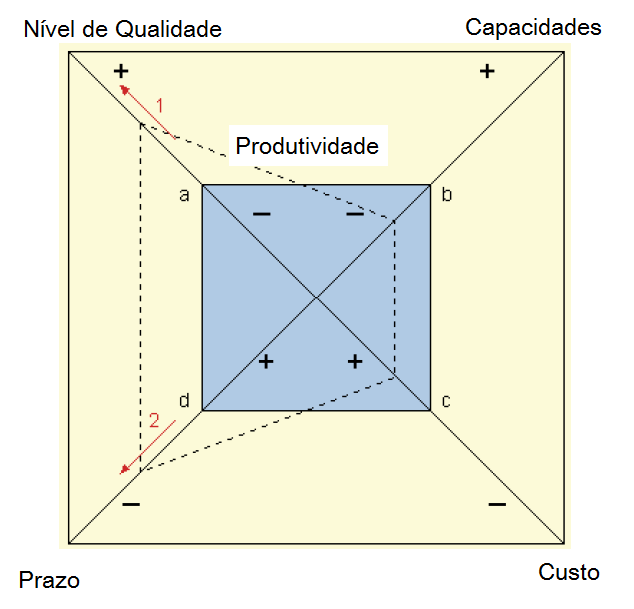
\includegraphics[scale=0.6]{devils_square.png}
 \caption{\label{fig:qpcs}\textit{The Devil's square}, adaptado de
 \cite{grunbacher2001surfacing} }
\end{figure*}
 
\FloatBarrier

A motivação deste trabalho é apresentar e comparar as técnicas de negociação de
requisitos, compilando todas as informações encontradas em um único
trabalho, visto que não encontramos nenhum com esta proposta, ainda que a
literatura sobre técnicas de negociação de requisitos seja ampla.
Entendemos que é de fundamental importância expor o conhecimento de forma
acessível, ou seja, fácil de se encontrar e de compreender, a fim de guiar os stakeholders
na sua busca por uma técnica adequada.

 \section{Objetivos}

Este trabalho visa apresentar um conjunto de técnicas de
negociação de requisitos encontradas na literatura, suas vantagens, suas
desvantagens e os achados importantes sobre cada uma. Para tal, buscamos realizar
uma revisão ampla, justa e quasi-sistemática da literatura.

\section{Organização da Monografia}

O restante deste trabalho está organizado da seguinte forma:
No Capítulo 2 descrevemos o planejamento, a execução e os dados extraídos da
revisão quasi-sistemática conduzida.
No capítulo 3 discutimos os resultados, respondendo as questãos de pesquisa.
Por fim, no capítulo 4 apresentamos as contribuições, limitações e perspectivas de trabalhos futuros.
